\documentclass[]{scrartcl}
\usepackage{lmodern}
\usepackage{amssymb,amsmath}
\usepackage{ifxetex,ifluatex}
\usepackage{fixltx2e} % provides \textsubscript
\ifnum 0\ifxetex 1\fi\ifluatex 1\fi=0 % if pdftex
  \usepackage[T1]{fontenc}
  \usepackage[utf8]{inputenc}
\else % if luatex or xelatex
  \ifxetex
    \usepackage{mathspec}
  \else
    \usepackage{fontspec}
  \fi
  \defaultfontfeatures{Ligatures=TeX,Scale=MatchLowercase}
\fi
% use upquote if available, for straight quotes in verbatim environments
\IfFileExists{upquote.sty}{\usepackage{upquote}}{}
% use microtype if available
\IfFileExists{microtype.sty}{%
\usepackage{microtype}
\UseMicrotypeSet[protrusion]{basicmath} % disable protrusion for tt fonts
}{}
\usepackage{hyperref}
\hypersetup{unicode=true,
            pdftitle={Biodose Tools},
            pdfauthor={Alfredo Hernández},
            pdfborder={0 0 0},
            breaklinks=true}
\urlstyle{same}  % don't use monospace font for urls
\usepackage{natbib}
\bibliographystyle{apalike}
\usepackage{longtable,booktabs}
\usepackage{graphicx,grffile}
\makeatletter
\def\maxwidth{\ifdim\Gin@nat@width>\linewidth\linewidth\else\Gin@nat@width\fi}
\def\maxheight{\ifdim\Gin@nat@height>\textheight\textheight\else\Gin@nat@height\fi}
\makeatother
% Scale images if necessary, so that they will not overflow the page
% margins by default, and it is still possible to overwrite the defaults
% using explicit options in \includegraphics[width, height, ...]{}
\setkeys{Gin}{width=\maxwidth,height=\maxheight,keepaspectratio}
\IfFileExists{parskip.sty}{%
\usepackage{parskip}
}{% else
\setlength{\parindent}{0pt}
\setlength{\parskip}{6pt plus 2pt minus 1pt}
}
\setlength{\emergencystretch}{3em}  % prevent overfull lines
\providecommand{\tightlist}{%
  \setlength{\itemsep}{0pt}\setlength{\parskip}{0pt}}
\setcounter{secnumdepth}{5}
% Redefines (sub)paragraphs to behave more like sections
\ifx\paragraph\undefined\else
\let\oldparagraph\paragraph
\renewcommand{\paragraph}[1]{\oldparagraph{#1}\mbox{}}
\fi
\ifx\subparagraph\undefined\else
\let\oldsubparagraph\subparagraph
\renewcommand{\subparagraph}[1]{\oldsubparagraph{#1}\mbox{}}
\fi

%%% Use protect on footnotes to avoid problems with footnotes in titles
\let\rmarkdownfootnote\footnote%
\def\footnote{\protect\rmarkdownfootnote}

%%% Change title format to be more compact
\usepackage{titling}

% Create subtitle command for use in maketitle
\providecommand{\subtitle}[1]{
  \posttitle{
    \begin{center}\large#1\end{center}
    }
}

\setlength{\droptitle}{-2em}

  \title{Biodose Tools}
    \pretitle{\vspace{\droptitle}\centering\huge}
  \posttitle{\par}
    \author{Alfredo Hernández}
    \preauthor{\centering\large\emph}
  \postauthor{\par}
      \predate{\centering\large\emph}
  \postdate{\par}
    \date{2019-07-01}

% \documentclass[paper=a4, fontsize=12pt, twoside=semi, abstracton, listof=totoc, toc=left]{scrartcl}
\usepackage[T1]{fontenc}
\usepackage[utf8]{inputenc}
% \usepackage{lmodern}
\usepackage{newpxtext}
\usepackage{newpxmath}
\let\openbox\relax
\usepackage{slantsc}
\usepackage{microtype}


% Sectioning layout
\addtokomafont{sectioning}{\normalfont\bfseries}
\setkomafont{section}{\LARGE}
\setkomafont{subsection}{\Large}
\setkomafont{subsubsection}{\large}
\setkomafont{paragraph}{\large}
\setkomafont{subparagraph}{\large}

\renewcommand\sectionformat
  {Chapter\enskip\thesection\autodot\hspace{1em}}


\usepackage{tocstyle}
\usetocstyle{standard}
% \renewcommand*\descriptionlabel[1]{\hspace\labelsep\normalfont\bfseries{#1}}
\usepackage[titletoc]{appendix}
\BeforeStartingTOC[lof]{\def\autodot{:}}
\BeforeStartingTOC[lot]{\def\autodot{:}}


% Empty pages
\usepackage{etoolbox}
\pretocmd{\toc}{\cleardoubleevenemptypage}{}{}
\pretocmd{\section}{\cleardoubleevenemptypage}{}{}
\pretocmd{\part}{\cleardoubleevenemptypage\thispagestyle{empty}}{}{}
\renewcommand\partheadstartvskip{\clearpage\null\vfil}
\renewcommand\partheadmidvskip{\par\nobreak\vskip 20pt\thispagestyle{empty}}

% Paragraph indentation behaviour
\setlength{\parindent}{0pt}
\setlength{\parskip}{0.3\baselineskip plus2pt minus2pt}
\newcommand{\sk}{\medskip\noindent}

% Fancy header and footer
% \usepackage{fancyhdr}
% \pagestyle{fancyplain}
% \fancyhead[LO]{\thepage}
% \fancyhead[CO]{}
% % \fancyhead[RO]{\nouppercase{ASD}}
% \fancyhead[RO]{\nouppercase{\rightmark}}
% \fancyhead[LE]{\nouppercase{\rightmark}}
% % % \fancyhead[LE]{\nouppercase{\leftmark}}
% \fancyhead[CE]{}
% \fancyhead[RE]{\thepage}
% \fancyfoot{}
% \renewcommand{\headrulewidth}{0.3pt}
% \renewcommand{\footrulewidth}{0pt}
% \setlength{\headheight}{13.6pt}

% Default packages
\usepackage{booktabs}
\usepackage{amsthm}
\makeatletter
\def\thm@space@setup{%
  \thm@preskip=8pt plus 2pt minus 4pt
  \thm@postskip=\thm@preskip
}
\makeatother

\begin{document}
\maketitle

{
\setcounter{tocdepth}{2}
\tableofcontents
}
\hypertarget{about}{%
\section{About}\label{about}}

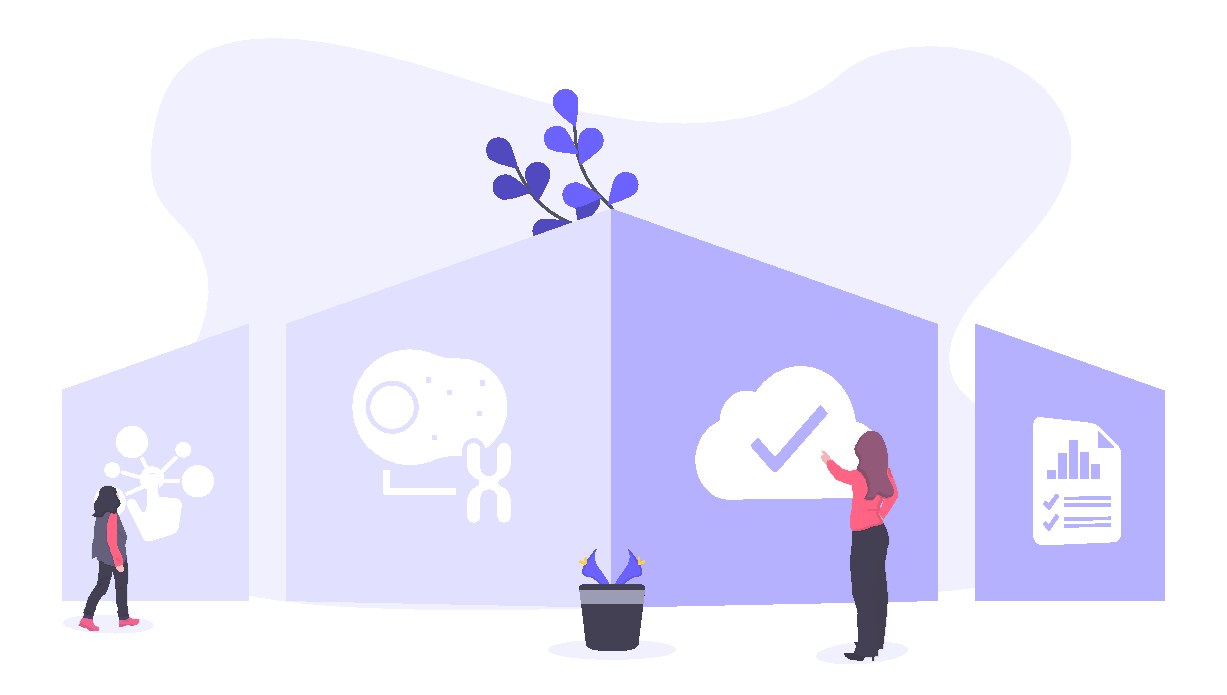
\includegraphics{assets/home.pdf}

This project in an app to be used by biological dosimetry laboratories. Biodose Tools is an open-source project that aims to be a tool to perform all different tests and calculations needed. The app is developed with \href{https://www.r-project.org/about.html}{R} \citep{R-base} together with \href{https://shiny.rstudio.com}{Shiny} to offer an on-line, easy-to-use solution. Although the intention is to provide the application as a website, all R routines can be downloaded for improvement or personal use.

We also aim to clarify and explain the tests used and to propose those considered most appropriate. Each laboratory in its routine work should choose the optimum method, but the project aims to reach a consensus that will help us in case of mutual assistance or intercomparisons.

The project is initially developed by \href{http://www.reneb.net}{RENEB} association, but contributions are always welcome.

\hypertarget{intro}{%
\section{Introduction}\label{intro}}

You can label chapter and section titles using \texttt{\{\#label\}} after them, e.g., we can reference Chapter \ref{intro}. If you do not manually label them, there will be automatic labels anyway, e.g., Chapter \ref{methods}.

\hypertarget{part-getting-biodose-tools}{%
\part{Getting Biodose Tools}\label{part-getting-biodose-tools}}

\hypertarget{online}{%
\section{Online}\label{online}}

Here is a review of existing methods.

\hypertarget{part-using-biodose-tools}{%
\part{Using Biodose Tools}\label{part-using-biodose-tools}}

\hypertarget{user-interface}{%
\section{User Interface}\label{user-interface}}

We describe our methods in this chapter.

\hypertarget{part-statistical-methods}{%
\part{Statistical Methods}\label{part-statistical-methods}}

\hypertarget{applications}{%
\section{Applications}\label{applications}}

Some \emph{significant} applications are demonstrated in this chapter.

\hypertarget{example-one}{%
\subsection{Example one}\label{example-one}}

\hypertarget{example-two}{%
\subsection{Example two}\label{example-two}}

\hypertarget{final-words}{%
\section{Final Words}\label{final-words}}

We have finished a nice book.

\hypertarget{refs}{}

\hypertarget{appendix-appendices}{%
\appendix}


\hypertarget{appendix-a-black-magic}{%
\section{Appendix A: Black Magic}\label{appendix-a-black-magic}}

\bibliography{book.bib,packages.bib}


\end{document}
